% Created by tikzDevice version 0.6.2-92-0ad2792 on 2013-01-10 17:41:47
% !TEX encoding = UTF-8 Unicode
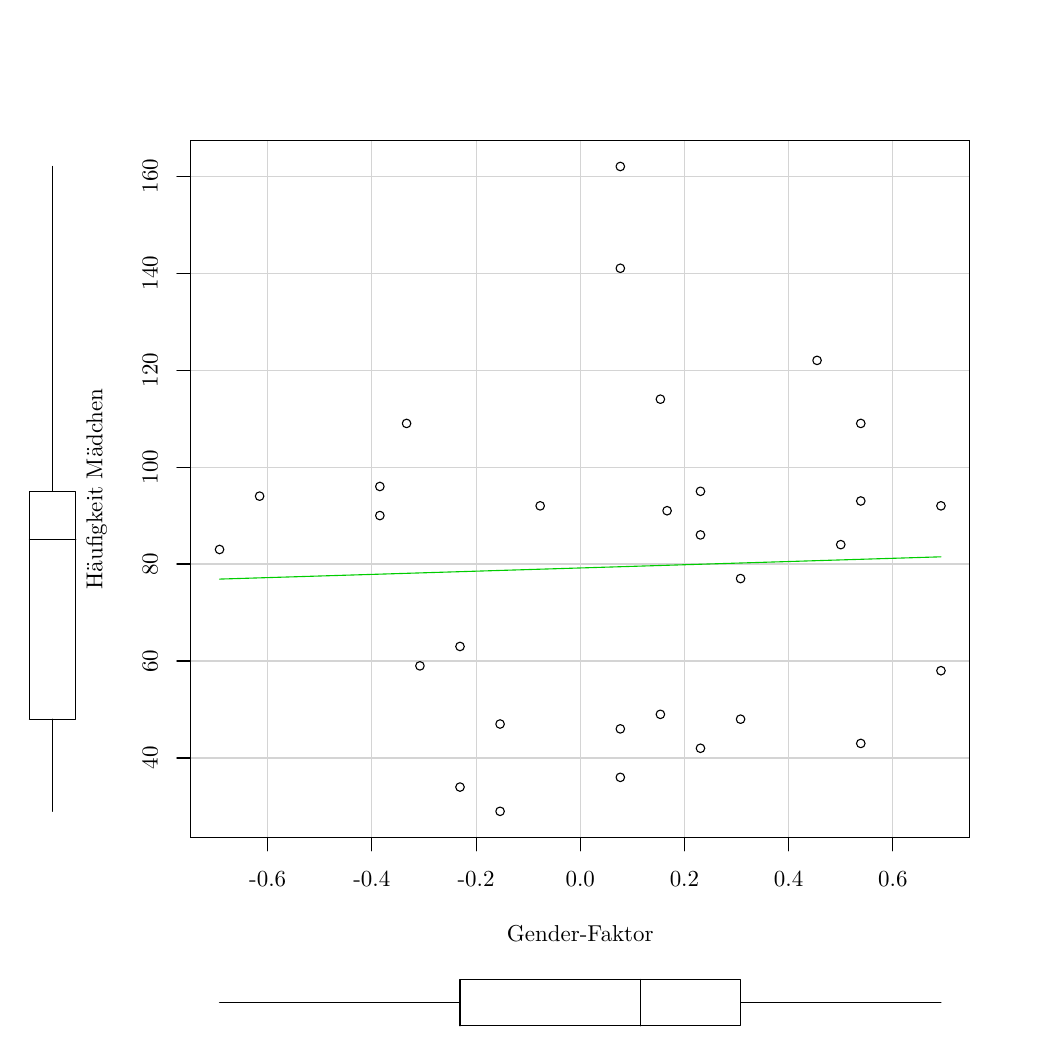
\begin{tikzpicture}[x=1pt,y=1pt]
\definecolor[named]{fillColor}{rgb}{1.00,1.00,1.00}
\path[use as bounding box,fill=fillColor,fill opacity=0.00] (0,0) rectangle (361.35,361.35);
\begin{scope}
\path[clip] (  0.00, 68.86) rectangle ( 18.07,320.51);
\definecolor[named]{drawColor}{rgb}{0.00,0.00,0.00}

\path[draw=drawColor,line width= 0.4pt,line join=round,line cap=round] (  0.67,111.47) --
	( 17.40,111.47) --
	( 17.40,193.81) --
	(  0.67,193.81) --
	(  0.67,111.47);

\path[draw=drawColor,line width= 0.4pt,line join=round,line cap=round] (  0.67,176.29) --
	( 17.40,176.29);

\path[draw=drawColor,line width= 0.4pt,line join=round,line cap=round] (  9.03, 78.18) --
	(  9.03,111.47);

\path[draw=drawColor,line width= 0.4pt,line join=round,line cap=round] (  9.03,193.81) --
	(  9.03,311.19);
\end{scope}
\begin{scope}
\path[clip] ( 58.90,  0.00) rectangle (340.43, 18.07);
\definecolor[named]{drawColor}{rgb}{0.00,0.00,0.00}

\path[draw=drawColor,line width= 0.4pt,line join=round,line cap=round] (156.22,  0.67) --
	(156.22, 17.40) --
	(257.60, 17.40) --
	(257.60,  0.67) --
	(156.22,  0.67);

\path[draw=drawColor,line width= 0.4pt,line join=round,line cap=round] (221.39,  0.67) --
	(221.39, 17.40);

\path[draw=drawColor,line width= 0.4pt,line join=round,line cap=round] ( 69.33,  9.03) --
	(156.22,  9.03);

\path[draw=drawColor,line width= 0.4pt,line join=round,line cap=round] (257.60,  9.03) --
	(330.01,  9.03);
\end{scope}
\begin{scope}
\path[clip] (  0.00,  0.00) rectangle (361.35,361.35);
\definecolor[named]{drawColor}{rgb}{0.00,0.00,0.00}

\path[draw=drawColor,line width= 0.4pt,line join=round,line cap=round] ( 86.71, 68.86) -- (312.63, 68.86);

\path[draw=drawColor,line width= 0.4pt,line join=round,line cap=round] ( 86.71, 68.86) -- ( 86.71, 63.88);

\path[draw=drawColor,line width= 0.4pt,line join=round,line cap=round] (124.36, 68.86) -- (124.36, 63.88);

\path[draw=drawColor,line width= 0.4pt,line join=round,line cap=round] (162.02, 68.86) -- (162.02, 63.88);

\path[draw=drawColor,line width= 0.4pt,line join=round,line cap=round] (199.67, 68.86) -- (199.67, 63.88);

\path[draw=drawColor,line width= 0.4pt,line join=round,line cap=round] (237.32, 68.86) -- (237.32, 63.88);

\path[draw=drawColor,line width= 0.4pt,line join=round,line cap=round] (274.98, 68.86) -- (274.98, 63.88);

\path[draw=drawColor,line width= 0.4pt,line join=round,line cap=round] (312.63, 68.86) -- (312.63, 63.88);

\node[text=drawColor,anchor=base,inner sep=0pt, outer sep=0pt, scale=  0.83] at ( 86.71, 50.94) {-0.6};

\node[text=drawColor,anchor=base,inner sep=0pt, outer sep=0pt, scale=  0.83] at (124.36, 50.94) {-0.4};

\node[text=drawColor,anchor=base,inner sep=0pt, outer sep=0pt, scale=  0.83] at (162.02, 50.94) {-0.2};

\node[text=drawColor,anchor=base,inner sep=0pt, outer sep=0pt, scale=  0.83] at (199.67, 50.94) {0.0};

\node[text=drawColor,anchor=base,inner sep=0pt, outer sep=0pt, scale=  0.83] at (237.32, 50.94) {0.2};

\node[text=drawColor,anchor=base,inner sep=0pt, outer sep=0pt, scale=  0.83] at (274.98, 50.94) {0.4};

\node[text=drawColor,anchor=base,inner sep=0pt, outer sep=0pt, scale=  0.83] at (312.63, 50.94) {0.6};

\path[draw=drawColor,line width= 0.4pt,line join=round,line cap=round] ( 58.90, 97.46) -- ( 58.90,307.69);

\path[draw=drawColor,line width= 0.4pt,line join=round,line cap=round] ( 58.90, 97.46) -- ( 53.92, 97.46);

\path[draw=drawColor,line width= 0.4pt,line join=round,line cap=round] ( 58.90,132.49) -- ( 53.92,132.49);

\path[draw=drawColor,line width= 0.4pt,line join=round,line cap=round] ( 58.90,167.53) -- ( 53.92,167.53);

\path[draw=drawColor,line width= 0.4pt,line join=round,line cap=round] ( 58.90,202.57) -- ( 53.92,202.57);

\path[draw=drawColor,line width= 0.4pt,line join=round,line cap=round] ( 58.90,237.61) -- ( 53.92,237.61);

\path[draw=drawColor,line width= 0.4pt,line join=round,line cap=round] ( 58.90,272.65) -- ( 53.92,272.65);

\path[draw=drawColor,line width= 0.4pt,line join=round,line cap=round] ( 58.90,307.69) -- ( 53.92,307.69);

\node[text=drawColor,rotate= 90.00,anchor=base,inner sep=0pt, outer sep=0pt, scale=  0.83] at ( 46.95, 97.46) {40};

\node[text=drawColor,rotate= 90.00,anchor=base,inner sep=0pt, outer sep=0pt, scale=  0.83] at ( 46.95,132.49) {60};

\node[text=drawColor,rotate= 90.00,anchor=base,inner sep=0pt, outer sep=0pt, scale=  0.83] at ( 46.95,167.53) {80};

\node[text=drawColor,rotate= 90.00,anchor=base,inner sep=0pt, outer sep=0pt, scale=  0.83] at ( 46.95,202.57) {100};

\node[text=drawColor,rotate= 90.00,anchor=base,inner sep=0pt, outer sep=0pt, scale=  0.83] at ( 46.95,237.61) {120};

\node[text=drawColor,rotate= 90.00,anchor=base,inner sep=0pt, outer sep=0pt, scale=  0.83] at ( 46.95,272.65) {140};

\node[text=drawColor,rotate= 90.00,anchor=base,inner sep=0pt, outer sep=0pt, scale=  0.83] at ( 46.95,307.69) {160};

\path[draw=drawColor,line width= 0.4pt,line join=round,line cap=round] ( 58.90, 68.86) --
	(340.43, 68.86) --
	(340.43,320.51) --
	( 58.90,320.51) --
	( 58.90, 68.86);
\end{scope}
\begin{scope}
\path[clip] ( 18.07, 18.07) rectangle (361.35,361.35);
\definecolor[named]{drawColor}{rgb}{0.00,0.00,0.00}

\node[text=drawColor,anchor=base,inner sep=0pt, outer sep=0pt, scale=  0.83] at (199.67, 31.02) {Gender-Faktor};

\node[text=drawColor,rotate= 90.00,anchor=base,inner sep=0pt, outer sep=0pt, scale=  0.83] at ( 27.03,194.69) {Häufigkeit Mädchen};
\end{scope}
\begin{scope}
\path[clip] ( 58.90, 68.86) rectangle (340.43,320.51);
\definecolor[named]{drawColor}{rgb}{0.83,0.83,0.83}

\path[draw=drawColor,line width= 0.4pt,line join=round,line cap=round] ( 86.71, 68.86) -- ( 86.71,320.51);

\path[draw=drawColor,line width= 0.4pt,line join=round,line cap=round] (124.36, 68.86) -- (124.36,320.51);

\path[draw=drawColor,line width= 0.4pt,line join=round,line cap=round] (162.02, 68.86) -- (162.02,320.51);

\path[draw=drawColor,line width= 0.4pt,line join=round,line cap=round] (199.67, 68.86) -- (199.67,320.51);

\path[draw=drawColor,line width= 0.4pt,line join=round,line cap=round] (237.32, 68.86) -- (237.32,320.51);

\path[draw=drawColor,line width= 0.4pt,line join=round,line cap=round] (274.98, 68.86) -- (274.98,320.51);

\path[draw=drawColor,line width= 0.4pt,line join=round,line cap=round] (312.63, 68.86) -- (312.63,320.51);

\path[draw=drawColor,line width= 0.4pt,line join=round,line cap=round] ( 58.90, 97.46) -- (340.43, 97.46);

\path[draw=drawColor,line width= 0.4pt,line join=round,line cap=round] ( 58.90,132.49) -- (340.43,132.49);

\path[draw=drawColor,line width= 0.4pt,line join=round,line cap=round] ( 58.90,167.53) -- (340.43,167.53);

\path[draw=drawColor,line width= 0.4pt,line join=round,line cap=round] ( 58.90,202.57) -- (340.43,202.57);

\path[draw=drawColor,line width= 0.4pt,line join=round,line cap=round] ( 58.90,237.61) -- (340.43,237.61);

\path[draw=drawColor,line width= 0.4pt,line join=round,line cap=round] ( 58.90,272.65) -- (340.43,272.65);

\path[draw=drawColor,line width= 0.4pt,line join=round,line cap=round] ( 58.90,307.69) -- (340.43,307.69);
\end{scope}
\begin{scope}
\path[clip] (  0.00,  0.00) rectangle (361.35,361.35);
\definecolor[named]{drawColor}{rgb}{0.00,0.00,0.00}

\path[draw=drawColor,line width= 0.4pt,line join=round,line cap=round] ( 58.90, 68.86) --
	(340.43, 68.86) --
	(340.43,320.51) --
	( 58.90,320.51) --
	( 58.90, 68.86);
\end{scope}
\begin{scope}
\path[clip] ( 58.90, 68.86) rectangle (340.43,320.51);
\definecolor[named]{drawColor}{rgb}{0.00,0.00,0.00}

\path[draw=drawColor,line width= 0.4pt,line join=round,line cap=round] (214.15,107.97) circle (  1.55);

\path[draw=drawColor,line width= 0.4pt,line join=round,line cap=round] (170.70, 78.18) circle (  1.55);

\path[draw=drawColor,line width= 0.4pt,line join=round,line cap=round] (170.70,109.72) circle (  1.55);

\path[draw=drawColor,line width= 0.4pt,line join=round,line cap=round] (228.63,227.10) circle (  1.55);

\path[draw=drawColor,line width= 0.4pt,line join=round,line cap=round] (228.63,113.22) circle (  1.55);

\path[draw=drawColor,line width= 0.4pt,line join=round,line cap=round] (257.60,111.47) circle (  1.55);

\path[draw=drawColor,line width= 0.4pt,line join=round,line cap=round] (293.80,174.54) circle (  1.55);

\path[draw=drawColor,line width= 0.4pt,line join=round,line cap=round] (136.91,218.34) circle (  1.55);

\path[draw=drawColor,line width= 0.4pt,line join=round,line cap=round] (214.15,311.19) circle (  1.55);

\path[draw=drawColor,line width= 0.4pt,line join=round,line cap=round] ( 83.81,192.06) circle (  1.55);

\path[draw=drawColor,line width= 0.4pt,line join=round,line cap=round] (214.15,274.40) circle (  1.55);

\path[draw=drawColor,line width= 0.4pt,line join=round,line cap=round] (141.74,130.74) circle (  1.55);

\path[draw=drawColor,line width= 0.4pt,line join=round,line cap=round] (257.60,162.28) circle (  1.55);

\path[draw=drawColor,line width= 0.4pt,line join=round,line cap=round] (301.04,218.34) circle (  1.55);

\path[draw=drawColor,line width= 0.4pt,line join=round,line cap=round] (231.05,186.80) circle (  1.55);

\path[draw=drawColor,line width= 0.4pt,line join=round,line cap=round] (156.22, 86.94) circle (  1.55);

\path[draw=drawColor,line width= 0.4pt,line join=round,line cap=round] (214.15, 90.45) circle (  1.55);

\path[draw=drawColor,line width= 0.4pt,line join=round,line cap=round] (185.19,188.56) circle (  1.55);

\path[draw=drawColor,line width= 0.4pt,line join=round,line cap=round] (243.11,100.96) circle (  1.55);

\path[draw=drawColor,line width= 0.4pt,line join=round,line cap=round] (127.26,195.56) circle (  1.55);

\path[draw=drawColor,line width= 0.4pt,line join=round,line cap=round] (330.01,188.56) circle (  1.55);

\path[draw=drawColor,line width= 0.4pt,line join=round,line cap=round] (127.26,185.05) circle (  1.55);

\path[draw=drawColor,line width= 0.4pt,line join=round,line cap=round] (301.04,102.71) circle (  1.55);

\path[draw=drawColor,line width= 0.4pt,line join=round,line cap=round] ( 69.33,172.79) circle (  1.55);

\path[draw=drawColor,line width= 0.4pt,line join=round,line cap=round] (243.11,193.81) circle (  1.55);

\path[draw=drawColor,line width= 0.4pt,line join=round,line cap=round] (301.04,190.31) circle (  1.55);

\path[draw=drawColor,line width= 0.4pt,line join=round,line cap=round] (243.11,178.05) circle (  1.55);

\path[draw=drawColor,line width= 0.4pt,line join=round,line cap=round] (330.01,128.99) circle (  1.55);

\path[draw=drawColor,line width= 0.4pt,line join=round,line cap=round] (285.24,241.12) circle (  1.55);

\path[draw=drawColor,line width= 0.4pt,line join=round,line cap=round] (156.22,137.75) circle (  1.55);
\definecolor[named]{drawColor}{rgb}{0.00,0.80,0.00}

\path[draw=drawColor,line width= 0.4pt,line join=round,line cap=round] ( 69.33,162.09) --
	(330.01,170.14);
\end{scope}
\end{tikzpicture}
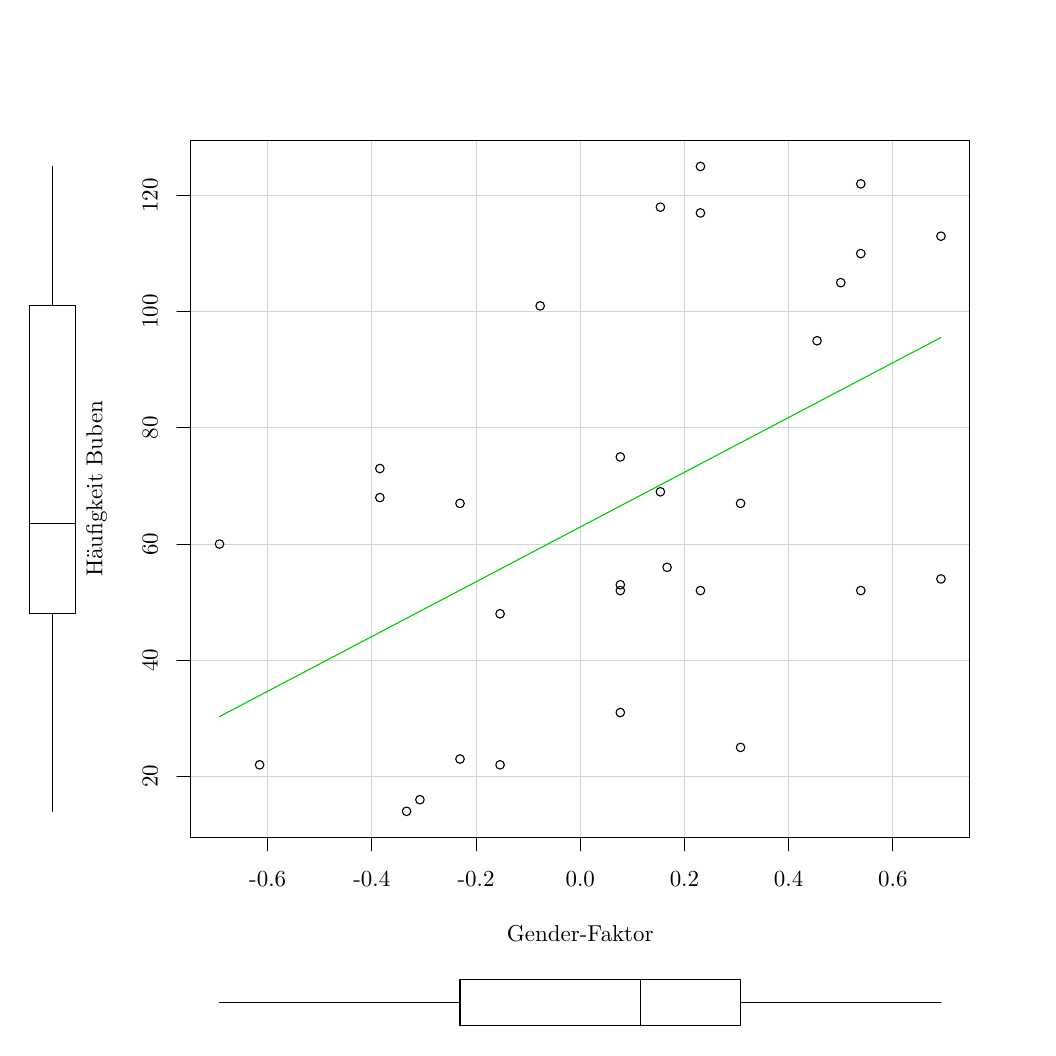
\begin{tikzpicture}[x=1pt,y=1pt]
\definecolor[named]{fillColor}{rgb}{1.00,1.00,1.00}
\path[use as bounding box,fill=fillColor,fill opacity=0.00] (0,0) rectangle (361.35,361.35);
\begin{scope}
\path[clip] (  0.00, 68.86) rectangle ( 18.07,320.51);
\definecolor[named]{drawColor}{rgb}{0.00,0.00,0.00}

\path[draw=drawColor,line width= 0.4pt,line join=round,line cap=round] (  0.67,149.56) --
	( 17.40,149.56) --
	( 17.40,260.81) --
	(  0.67,260.81) --
	(  0.67,149.56);

\path[draw=drawColor,line width= 0.4pt,line join=round,line cap=round] (  0.67,182.09) --
	( 17.40,182.09);

\path[draw=drawColor,line width= 0.4pt,line join=round,line cap=round] (  9.03, 78.18) --
	(  9.03,149.56);

\path[draw=drawColor,line width= 0.4pt,line join=round,line cap=round] (  9.03,260.81) --
	(  9.03,311.19);
\end{scope}
\begin{scope}
\path[clip] ( 58.90,  0.00) rectangle (340.43, 18.07);
\definecolor[named]{drawColor}{rgb}{0.00,0.00,0.00}

\path[draw=drawColor,line width= 0.4pt,line join=round,line cap=round] (156.22,  0.67) --
	(156.22, 17.40) --
	(257.60, 17.40) --
	(257.60,  0.67) --
	(156.22,  0.67);

\path[draw=drawColor,line width= 0.4pt,line join=round,line cap=round] (221.39,  0.67) --
	(221.39, 17.40);

\path[draw=drawColor,line width= 0.4pt,line join=round,line cap=round] ( 69.33,  9.03) --
	(156.22,  9.03);

\path[draw=drawColor,line width= 0.4pt,line join=round,line cap=round] (257.60,  9.03) --
	(330.01,  9.03);
\end{scope}
\begin{scope}
\path[clip] (  0.00,  0.00) rectangle (361.35,361.35);
\definecolor[named]{drawColor}{rgb}{0.00,0.00,0.00}

\path[draw=drawColor,line width= 0.4pt,line join=round,line cap=round] ( 86.71, 68.86) -- (312.63, 68.86);

\path[draw=drawColor,line width= 0.4pt,line join=round,line cap=round] ( 86.71, 68.86) -- ( 86.71, 63.88);

\path[draw=drawColor,line width= 0.4pt,line join=round,line cap=round] (124.36, 68.86) -- (124.36, 63.88);

\path[draw=drawColor,line width= 0.4pt,line join=round,line cap=round] (162.02, 68.86) -- (162.02, 63.88);

\path[draw=drawColor,line width= 0.4pt,line join=round,line cap=round] (199.67, 68.86) -- (199.67, 63.88);

\path[draw=drawColor,line width= 0.4pt,line join=round,line cap=round] (237.32, 68.86) -- (237.32, 63.88);

\path[draw=drawColor,line width= 0.4pt,line join=round,line cap=round] (274.98, 68.86) -- (274.98, 63.88);

\path[draw=drawColor,line width= 0.4pt,line join=round,line cap=round] (312.63, 68.86) -- (312.63, 63.88);

\node[text=drawColor,anchor=base,inner sep=0pt, outer sep=0pt, scale=  0.83] at ( 86.71, 50.94) {-0.6};

\node[text=drawColor,anchor=base,inner sep=0pt, outer sep=0pt, scale=  0.83] at (124.36, 50.94) {-0.4};

\node[text=drawColor,anchor=base,inner sep=0pt, outer sep=0pt, scale=  0.83] at (162.02, 50.94) {-0.2};

\node[text=drawColor,anchor=base,inner sep=0pt, outer sep=0pt, scale=  0.83] at (199.67, 50.94) {0.0};

\node[text=drawColor,anchor=base,inner sep=0pt, outer sep=0pt, scale=  0.83] at (237.32, 50.94) {0.2};

\node[text=drawColor,anchor=base,inner sep=0pt, outer sep=0pt, scale=  0.83] at (274.98, 50.94) {0.4};

\node[text=drawColor,anchor=base,inner sep=0pt, outer sep=0pt, scale=  0.83] at (312.63, 50.94) {0.6};

\path[draw=drawColor,line width= 0.4pt,line join=round,line cap=round] ( 58.90, 90.78) -- ( 58.90,300.70);

\path[draw=drawColor,line width= 0.4pt,line join=round,line cap=round] ( 58.90, 90.78) -- ( 53.92, 90.78);

\path[draw=drawColor,line width= 0.4pt,line join=round,line cap=round] ( 58.90,132.76) -- ( 53.92,132.76);

\path[draw=drawColor,line width= 0.4pt,line join=round,line cap=round] ( 58.90,174.75) -- ( 53.92,174.75);

\path[draw=drawColor,line width= 0.4pt,line join=round,line cap=round] ( 58.90,216.73) -- ( 53.92,216.73);

\path[draw=drawColor,line width= 0.4pt,line join=round,line cap=round] ( 58.90,258.71) -- ( 53.92,258.71);

\path[draw=drawColor,line width= 0.4pt,line join=round,line cap=round] ( 58.90,300.70) -- ( 53.92,300.70);

\node[text=drawColor,rotate= 90.00,anchor=base,inner sep=0pt, outer sep=0pt, scale=  0.83] at ( 46.95, 90.78) {20};

\node[text=drawColor,rotate= 90.00,anchor=base,inner sep=0pt, outer sep=0pt, scale=  0.83] at ( 46.95,132.76) {40};

\node[text=drawColor,rotate= 90.00,anchor=base,inner sep=0pt, outer sep=0pt, scale=  0.83] at ( 46.95,174.75) {60};

\node[text=drawColor,rotate= 90.00,anchor=base,inner sep=0pt, outer sep=0pt, scale=  0.83] at ( 46.95,216.73) {80};

\node[text=drawColor,rotate= 90.00,anchor=base,inner sep=0pt, outer sep=0pt, scale=  0.83] at ( 46.95,258.71) {100};

\node[text=drawColor,rotate= 90.00,anchor=base,inner sep=0pt, outer sep=0pt, scale=  0.83] at ( 46.95,300.70) {120};

\path[draw=drawColor,line width= 0.4pt,line join=round,line cap=round] ( 58.90, 68.86) --
	(340.43, 68.86) --
	(340.43,320.51) --
	( 58.90,320.51) --
	( 58.90, 68.86);
\end{scope}
\begin{scope}
\path[clip] ( 18.07, 18.07) rectangle (361.35,361.35);
\definecolor[named]{drawColor}{rgb}{0.00,0.00,0.00}

\node[text=drawColor,anchor=base,inner sep=0pt, outer sep=0pt, scale=  0.83] at (199.67, 31.02) {Gender-Faktor};

\node[text=drawColor,rotate= 90.00,anchor=base,inner sep=0pt, outer sep=0pt, scale=  0.83] at ( 27.03,194.69) {Häufigkeit Buben};
\end{scope}
\begin{scope}
\path[clip] ( 58.90, 68.86) rectangle (340.43,320.51);
\definecolor[named]{drawColor}{rgb}{0.83,0.83,0.83}

\path[draw=drawColor,line width= 0.4pt,line join=round,line cap=round] ( 86.71, 68.86) -- ( 86.71,320.51);

\path[draw=drawColor,line width= 0.4pt,line join=round,line cap=round] (124.36, 68.86) -- (124.36,320.51);

\path[draw=drawColor,line width= 0.4pt,line join=round,line cap=round] (162.02, 68.86) -- (162.02,320.51);

\path[draw=drawColor,line width= 0.4pt,line join=round,line cap=round] (199.67, 68.86) -- (199.67,320.51);

\path[draw=drawColor,line width= 0.4pt,line join=round,line cap=round] (237.32, 68.86) -- (237.32,320.51);

\path[draw=drawColor,line width= 0.4pt,line join=round,line cap=round] (274.98, 68.86) -- (274.98,320.51);

\path[draw=drawColor,line width= 0.4pt,line join=round,line cap=round] (312.63, 68.86) -- (312.63,320.51);

\path[draw=drawColor,line width= 0.4pt,line join=round,line cap=round] ( 58.90, 90.78) -- (340.43, 90.78);

\path[draw=drawColor,line width= 0.4pt,line join=round,line cap=round] ( 58.90,132.76) -- (340.43,132.76);

\path[draw=drawColor,line width= 0.4pt,line join=round,line cap=round] ( 58.90,174.75) -- (340.43,174.75);

\path[draw=drawColor,line width= 0.4pt,line join=round,line cap=round] ( 58.90,216.73) -- (340.43,216.73);

\path[draw=drawColor,line width= 0.4pt,line join=round,line cap=round] ( 58.90,258.71) -- (340.43,258.71);

\path[draw=drawColor,line width= 0.4pt,line join=round,line cap=round] ( 58.90,300.70) -- (340.43,300.70);
\end{scope}
\begin{scope}
\path[clip] (  0.00,  0.00) rectangle (361.35,361.35);
\definecolor[named]{drawColor}{rgb}{0.00,0.00,0.00}

\path[draw=drawColor,line width= 0.4pt,line join=round,line cap=round] ( 58.90, 68.86) --
	(340.43, 68.86) --
	(340.43,320.51) --
	( 58.90,320.51) --
	( 58.90, 68.86);
\end{scope}
\begin{scope}
\path[clip] ( 58.90, 68.86) rectangle (340.43,320.51);
\definecolor[named]{drawColor}{rgb}{0.00,0.00,0.00}

\path[draw=drawColor,line width= 0.4pt,line join=round,line cap=round] (214.15,157.95) circle (  1.55);

\path[draw=drawColor,line width= 0.4pt,line join=round,line cap=round] (170.70, 94.98) circle (  1.55);

\path[draw=drawColor,line width= 0.4pt,line join=round,line cap=round] (170.70,149.56) circle (  1.55);

\path[draw=drawColor,line width= 0.4pt,line join=round,line cap=round] (228.63,296.50) circle (  1.55);

\path[draw=drawColor,line width= 0.4pt,line join=round,line cap=round] (228.63,193.64) circle (  1.55);

\path[draw=drawColor,line width= 0.4pt,line join=round,line cap=round] (257.60,189.44) circle (  1.55);

\path[draw=drawColor,line width= 0.4pt,line join=round,line cap=round] (293.80,269.21) circle (  1.55);

\path[draw=drawColor,line width= 0.4pt,line join=round,line cap=round] (136.91, 78.18) circle (  1.55);

\path[draw=drawColor,line width= 0.4pt,line join=round,line cap=round] (214.15,160.05) circle (  1.55);

\path[draw=drawColor,line width= 0.4pt,line join=round,line cap=round] ( 83.81, 94.98) circle (  1.55);

\path[draw=drawColor,line width= 0.4pt,line join=round,line cap=round] (214.15,206.23) circle (  1.55);

\path[draw=drawColor,line width= 0.4pt,line join=round,line cap=round] (141.74, 82.38) circle (  1.55);

\path[draw=drawColor,line width= 0.4pt,line join=round,line cap=round] (257.60,101.27) circle (  1.55);

\path[draw=drawColor,line width= 0.4pt,line join=round,line cap=round] (301.04,157.95) circle (  1.55);

\path[draw=drawColor,line width= 0.4pt,line join=round,line cap=round] (231.05,166.35) circle (  1.55);

\path[draw=drawColor,line width= 0.4pt,line join=round,line cap=round] (156.22, 97.08) circle (  1.55);

\path[draw=drawColor,line width= 0.4pt,line join=round,line cap=round] (214.15,113.87) circle (  1.55);

\path[draw=drawColor,line width= 0.4pt,line join=round,line cap=round] (185.19,260.81) circle (  1.55);

\path[draw=drawColor,line width= 0.4pt,line join=round,line cap=round] (243.11,157.95) circle (  1.55);

\path[draw=drawColor,line width= 0.4pt,line join=round,line cap=round] (127.26,191.54) circle (  1.55);

\path[draw=drawColor,line width= 0.4pt,line join=round,line cap=round] (330.01,286.00) circle (  1.55);

\path[draw=drawColor,line width= 0.4pt,line join=round,line cap=round] (127.26,202.04) circle (  1.55);

\path[draw=drawColor,line width= 0.4pt,line join=round,line cap=round] (301.04,279.71) circle (  1.55);

\path[draw=drawColor,line width= 0.4pt,line join=round,line cap=round] ( 69.33,174.75) circle (  1.55);

\path[draw=drawColor,line width= 0.4pt,line join=round,line cap=round] (243.11,311.19) circle (  1.55);

\path[draw=drawColor,line width= 0.4pt,line join=round,line cap=round] (301.04,304.90) circle (  1.55);

\path[draw=drawColor,line width= 0.4pt,line join=round,line cap=round] (243.11,294.40) circle (  1.55);

\path[draw=drawColor,line width= 0.4pt,line join=round,line cap=round] (330.01,162.15) circle (  1.55);

\path[draw=drawColor,line width= 0.4pt,line join=round,line cap=round] (285.24,248.22) circle (  1.55);

\path[draw=drawColor,line width= 0.4pt,line join=round,line cap=round] (156.22,189.44) circle (  1.55);
\definecolor[named]{drawColor}{rgb}{0.00,0.80,0.00}

\path[draw=drawColor,line width= 0.4pt,line join=round,line cap=round] ( 69.33,112.42) --
	(330.01,249.40);
\end{scope}
\end{tikzpicture}
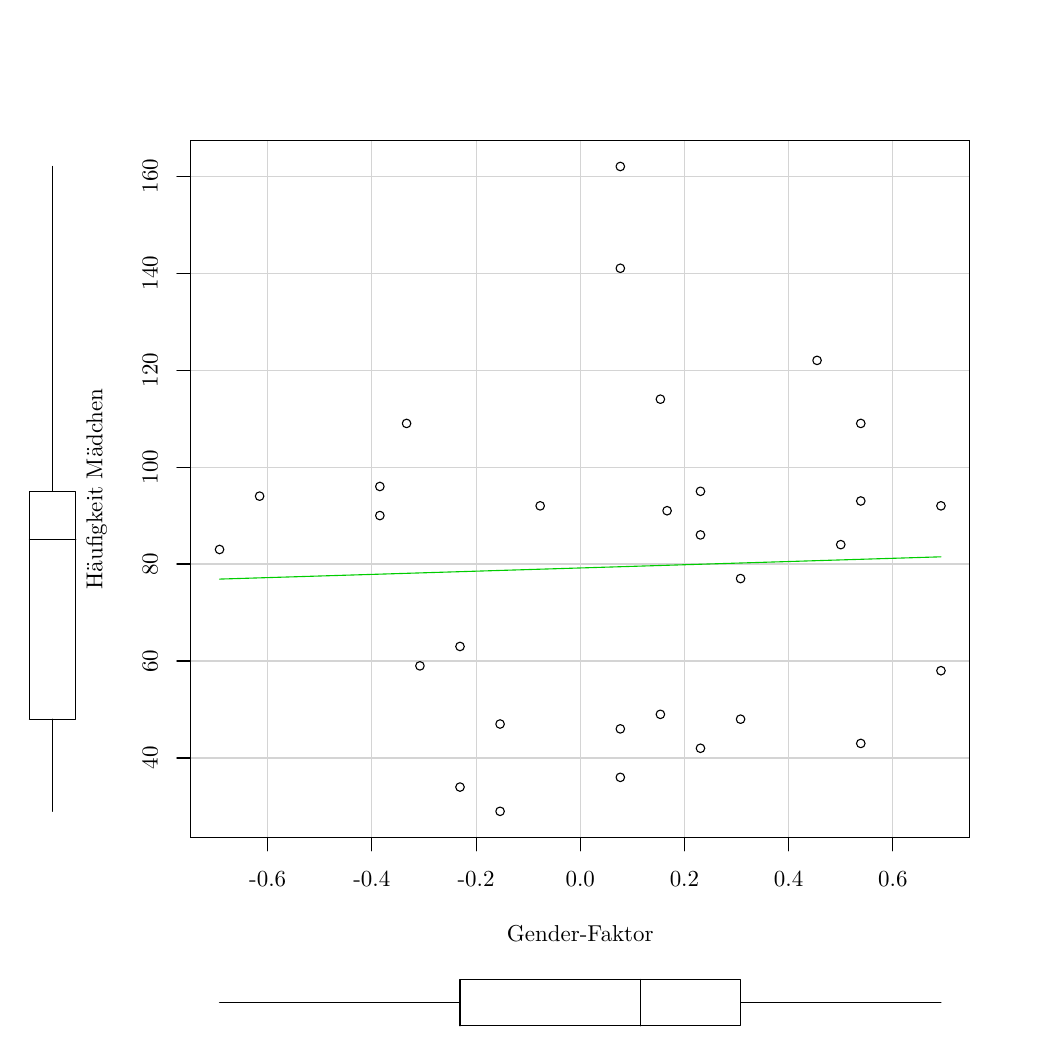
\begin{tikzpicture}[x=1pt,y=1pt]
\definecolor[named]{fillColor}{rgb}{1.00,1.00,1.00}
\path[use as bounding box,fill=fillColor,fill opacity=0.00] (0,0) rectangle (361.35,361.35);
\begin{scope}
\path[clip] (  0.00, 68.86) rectangle ( 18.07,320.51);
\definecolor[named]{drawColor}{rgb}{0.00,0.00,0.00}

\path[draw=drawColor,line width= 0.4pt,line join=round,line cap=round] (  0.67,111.47) --
	( 17.40,111.47) --
	( 17.40,193.81) --
	(  0.67,193.81) --
	(  0.67,111.47);

\path[draw=drawColor,line width= 0.4pt,line join=round,line cap=round] (  0.67,176.29) --
	( 17.40,176.29);

\path[draw=drawColor,line width= 0.4pt,line join=round,line cap=round] (  9.03, 78.18) --
	(  9.03,111.47);

\path[draw=drawColor,line width= 0.4pt,line join=round,line cap=round] (  9.03,193.81) --
	(  9.03,311.19);
\end{scope}
\begin{scope}
\path[clip] ( 58.90,  0.00) rectangle (340.43, 18.07);
\definecolor[named]{drawColor}{rgb}{0.00,0.00,0.00}

\path[draw=drawColor,line width= 0.4pt,line join=round,line cap=round] (156.22,  0.67) --
	(156.22, 17.40) --
	(257.60, 17.40) --
	(257.60,  0.67) --
	(156.22,  0.67);

\path[draw=drawColor,line width= 0.4pt,line join=round,line cap=round] (221.39,  0.67) --
	(221.39, 17.40);

\path[draw=drawColor,line width= 0.4pt,line join=round,line cap=round] ( 69.33,  9.03) --
	(156.22,  9.03);

\path[draw=drawColor,line width= 0.4pt,line join=round,line cap=round] (257.60,  9.03) --
	(330.01,  9.03);
\end{scope}
\begin{scope}
\path[clip] (  0.00,  0.00) rectangle (361.35,361.35);
\definecolor[named]{drawColor}{rgb}{0.00,0.00,0.00}

\path[draw=drawColor,line width= 0.4pt,line join=round,line cap=round] ( 86.71, 68.86) -- (312.63, 68.86);

\path[draw=drawColor,line width= 0.4pt,line join=round,line cap=round] ( 86.71, 68.86) -- ( 86.71, 63.88);

\path[draw=drawColor,line width= 0.4pt,line join=round,line cap=round] (124.36, 68.86) -- (124.36, 63.88);

\path[draw=drawColor,line width= 0.4pt,line join=round,line cap=round] (162.02, 68.86) -- (162.02, 63.88);

\path[draw=drawColor,line width= 0.4pt,line join=round,line cap=round] (199.67, 68.86) -- (199.67, 63.88);

\path[draw=drawColor,line width= 0.4pt,line join=round,line cap=round] (237.32, 68.86) -- (237.32, 63.88);

\path[draw=drawColor,line width= 0.4pt,line join=round,line cap=round] (274.98, 68.86) -- (274.98, 63.88);

\path[draw=drawColor,line width= 0.4pt,line join=round,line cap=round] (312.63, 68.86) -- (312.63, 63.88);

\node[text=drawColor,anchor=base,inner sep=0pt, outer sep=0pt, scale=  0.83] at ( 86.71, 50.94) {-0.6};

\node[text=drawColor,anchor=base,inner sep=0pt, outer sep=0pt, scale=  0.83] at (124.36, 50.94) {-0.4};

\node[text=drawColor,anchor=base,inner sep=0pt, outer sep=0pt, scale=  0.83] at (162.02, 50.94) {-0.2};

\node[text=drawColor,anchor=base,inner sep=0pt, outer sep=0pt, scale=  0.83] at (199.67, 50.94) {0.0};

\node[text=drawColor,anchor=base,inner sep=0pt, outer sep=0pt, scale=  0.83] at (237.32, 50.94) {0.2};

\node[text=drawColor,anchor=base,inner sep=0pt, outer sep=0pt, scale=  0.83] at (274.98, 50.94) {0.4};

\node[text=drawColor,anchor=base,inner sep=0pt, outer sep=0pt, scale=  0.83] at (312.63, 50.94) {0.6};

\path[draw=drawColor,line width= 0.4pt,line join=round,line cap=round] ( 58.90, 97.46) -- ( 58.90,307.69);

\path[draw=drawColor,line width= 0.4pt,line join=round,line cap=round] ( 58.90, 97.46) -- ( 53.92, 97.46);

\path[draw=drawColor,line width= 0.4pt,line join=round,line cap=round] ( 58.90,132.49) -- ( 53.92,132.49);

\path[draw=drawColor,line width= 0.4pt,line join=round,line cap=round] ( 58.90,167.53) -- ( 53.92,167.53);

\path[draw=drawColor,line width= 0.4pt,line join=round,line cap=round] ( 58.90,202.57) -- ( 53.92,202.57);

\path[draw=drawColor,line width= 0.4pt,line join=round,line cap=round] ( 58.90,237.61) -- ( 53.92,237.61);

\path[draw=drawColor,line width= 0.4pt,line join=round,line cap=round] ( 58.90,272.65) -- ( 53.92,272.65);

\path[draw=drawColor,line width= 0.4pt,line join=round,line cap=round] ( 58.90,307.69) -- ( 53.92,307.69);

\node[text=drawColor,rotate= 90.00,anchor=base,inner sep=0pt, outer sep=0pt, scale=  0.83] at ( 46.95, 97.46) {40};

\node[text=drawColor,rotate= 90.00,anchor=base,inner sep=0pt, outer sep=0pt, scale=  0.83] at ( 46.95,132.49) {60};

\node[text=drawColor,rotate= 90.00,anchor=base,inner sep=0pt, outer sep=0pt, scale=  0.83] at ( 46.95,167.53) {80};

\node[text=drawColor,rotate= 90.00,anchor=base,inner sep=0pt, outer sep=0pt, scale=  0.83] at ( 46.95,202.57) {100};

\node[text=drawColor,rotate= 90.00,anchor=base,inner sep=0pt, outer sep=0pt, scale=  0.83] at ( 46.95,237.61) {120};

\node[text=drawColor,rotate= 90.00,anchor=base,inner sep=0pt, outer sep=0pt, scale=  0.83] at ( 46.95,272.65) {140};

\node[text=drawColor,rotate= 90.00,anchor=base,inner sep=0pt, outer sep=0pt, scale=  0.83] at ( 46.95,307.69) {160};

\path[draw=drawColor,line width= 0.4pt,line join=round,line cap=round] ( 58.90, 68.86) --
	(340.43, 68.86) --
	(340.43,320.51) --
	( 58.90,320.51) --
	( 58.90, 68.86);
\end{scope}
\begin{scope}
\path[clip] ( 18.07, 18.07) rectangle (361.35,361.35);
\definecolor[named]{drawColor}{rgb}{0.00,0.00,0.00}

\node[text=drawColor,anchor=base,inner sep=0pt, outer sep=0pt, scale=  0.83] at (199.67, 31.02) {Gender-Faktor};

\node[text=drawColor,rotate= 90.00,anchor=base,inner sep=0pt, outer sep=0pt, scale=  0.83] at ( 27.03,194.69) {Häufigkeit Mädchen};
\end{scope}
\begin{scope}
\path[clip] ( 58.90, 68.86) rectangle (340.43,320.51);
\definecolor[named]{drawColor}{rgb}{0.83,0.83,0.83}

\path[draw=drawColor,line width= 0.4pt,line join=round,line cap=round] ( 86.71, 68.86) -- ( 86.71,320.51);

\path[draw=drawColor,line width= 0.4pt,line join=round,line cap=round] (124.36, 68.86) -- (124.36,320.51);

\path[draw=drawColor,line width= 0.4pt,line join=round,line cap=round] (162.02, 68.86) -- (162.02,320.51);

\path[draw=drawColor,line width= 0.4pt,line join=round,line cap=round] (199.67, 68.86) -- (199.67,320.51);

\path[draw=drawColor,line width= 0.4pt,line join=round,line cap=round] (237.32, 68.86) -- (237.32,320.51);

\path[draw=drawColor,line width= 0.4pt,line join=round,line cap=round] (274.98, 68.86) -- (274.98,320.51);

\path[draw=drawColor,line width= 0.4pt,line join=round,line cap=round] (312.63, 68.86) -- (312.63,320.51);

\path[draw=drawColor,line width= 0.4pt,line join=round,line cap=round] ( 58.90, 97.46) -- (340.43, 97.46);

\path[draw=drawColor,line width= 0.4pt,line join=round,line cap=round] ( 58.90,132.49) -- (340.43,132.49);

\path[draw=drawColor,line width= 0.4pt,line join=round,line cap=round] ( 58.90,167.53) -- (340.43,167.53);

\path[draw=drawColor,line width= 0.4pt,line join=round,line cap=round] ( 58.90,202.57) -- (340.43,202.57);

\path[draw=drawColor,line width= 0.4pt,line join=round,line cap=round] ( 58.90,237.61) -- (340.43,237.61);

\path[draw=drawColor,line width= 0.4pt,line join=round,line cap=round] ( 58.90,272.65) -- (340.43,272.65);

\path[draw=drawColor,line width= 0.4pt,line join=round,line cap=round] ( 58.90,307.69) -- (340.43,307.69);
\end{scope}
\begin{scope}
\path[clip] (  0.00,  0.00) rectangle (361.35,361.35);
\definecolor[named]{drawColor}{rgb}{0.00,0.00,0.00}

\path[draw=drawColor,line width= 0.4pt,line join=round,line cap=round] ( 58.90, 68.86) --
	(340.43, 68.86) --
	(340.43,320.51) --
	( 58.90,320.51) --
	( 58.90, 68.86);
\end{scope}
\begin{scope}
\path[clip] ( 58.90, 68.86) rectangle (340.43,320.51);
\definecolor[named]{drawColor}{rgb}{0.00,0.00,0.00}

\path[draw=drawColor,line width= 0.4pt,line join=round,line cap=round] (214.15,107.97) circle (  1.55);

\path[draw=drawColor,line width= 0.4pt,line join=round,line cap=round] (170.70, 78.18) circle (  1.55);

\path[draw=drawColor,line width= 0.4pt,line join=round,line cap=round] (170.70,109.72) circle (  1.55);

\path[draw=drawColor,line width= 0.4pt,line join=round,line cap=round] (228.63,227.10) circle (  1.55);

\path[draw=drawColor,line width= 0.4pt,line join=round,line cap=round] (228.63,113.22) circle (  1.55);

\path[draw=drawColor,line width= 0.4pt,line join=round,line cap=round] (257.60,111.47) circle (  1.55);

\path[draw=drawColor,line width= 0.4pt,line join=round,line cap=round] (293.80,174.54) circle (  1.55);

\path[draw=drawColor,line width= 0.4pt,line join=round,line cap=round] (136.91,218.34) circle (  1.55);

\path[draw=drawColor,line width= 0.4pt,line join=round,line cap=round] (214.15,311.19) circle (  1.55);

\path[draw=drawColor,line width= 0.4pt,line join=round,line cap=round] ( 83.81,192.06) circle (  1.55);

\path[draw=drawColor,line width= 0.4pt,line join=round,line cap=round] (214.15,274.40) circle (  1.55);

\path[draw=drawColor,line width= 0.4pt,line join=round,line cap=round] (141.74,130.74) circle (  1.55);

\path[draw=drawColor,line width= 0.4pt,line join=round,line cap=round] (257.60,162.28) circle (  1.55);

\path[draw=drawColor,line width= 0.4pt,line join=round,line cap=round] (301.04,218.34) circle (  1.55);

\path[draw=drawColor,line width= 0.4pt,line join=round,line cap=round] (231.05,186.80) circle (  1.55);

\path[draw=drawColor,line width= 0.4pt,line join=round,line cap=round] (156.22, 86.94) circle (  1.55);

\path[draw=drawColor,line width= 0.4pt,line join=round,line cap=round] (214.15, 90.45) circle (  1.55);

\path[draw=drawColor,line width= 0.4pt,line join=round,line cap=round] (185.19,188.56) circle (  1.55);

\path[draw=drawColor,line width= 0.4pt,line join=round,line cap=round] (243.11,100.96) circle (  1.55);

\path[draw=drawColor,line width= 0.4pt,line join=round,line cap=round] (127.26,195.56) circle (  1.55);

\path[draw=drawColor,line width= 0.4pt,line join=round,line cap=round] (330.01,188.56) circle (  1.55);

\path[draw=drawColor,line width= 0.4pt,line join=round,line cap=round] (127.26,185.05) circle (  1.55);

\path[draw=drawColor,line width= 0.4pt,line join=round,line cap=round] (301.04,102.71) circle (  1.55);

\path[draw=drawColor,line width= 0.4pt,line join=round,line cap=round] ( 69.33,172.79) circle (  1.55);

\path[draw=drawColor,line width= 0.4pt,line join=round,line cap=round] (243.11,193.81) circle (  1.55);

\path[draw=drawColor,line width= 0.4pt,line join=round,line cap=round] (301.04,190.31) circle (  1.55);

\path[draw=drawColor,line width= 0.4pt,line join=round,line cap=round] (243.11,178.05) circle (  1.55);

\path[draw=drawColor,line width= 0.4pt,line join=round,line cap=round] (330.01,128.99) circle (  1.55);

\path[draw=drawColor,line width= 0.4pt,line join=round,line cap=round] (285.24,241.12) circle (  1.55);

\path[draw=drawColor,line width= 0.4pt,line join=round,line cap=round] (156.22,137.75) circle (  1.55);
\definecolor[named]{drawColor}{rgb}{0.00,0.80,0.00}

\path[draw=drawColor,line width= 0.4pt,line join=round,line cap=round] ( 69.33,162.09) --
	(330.01,170.14);
\end{scope}
\end{tikzpicture}
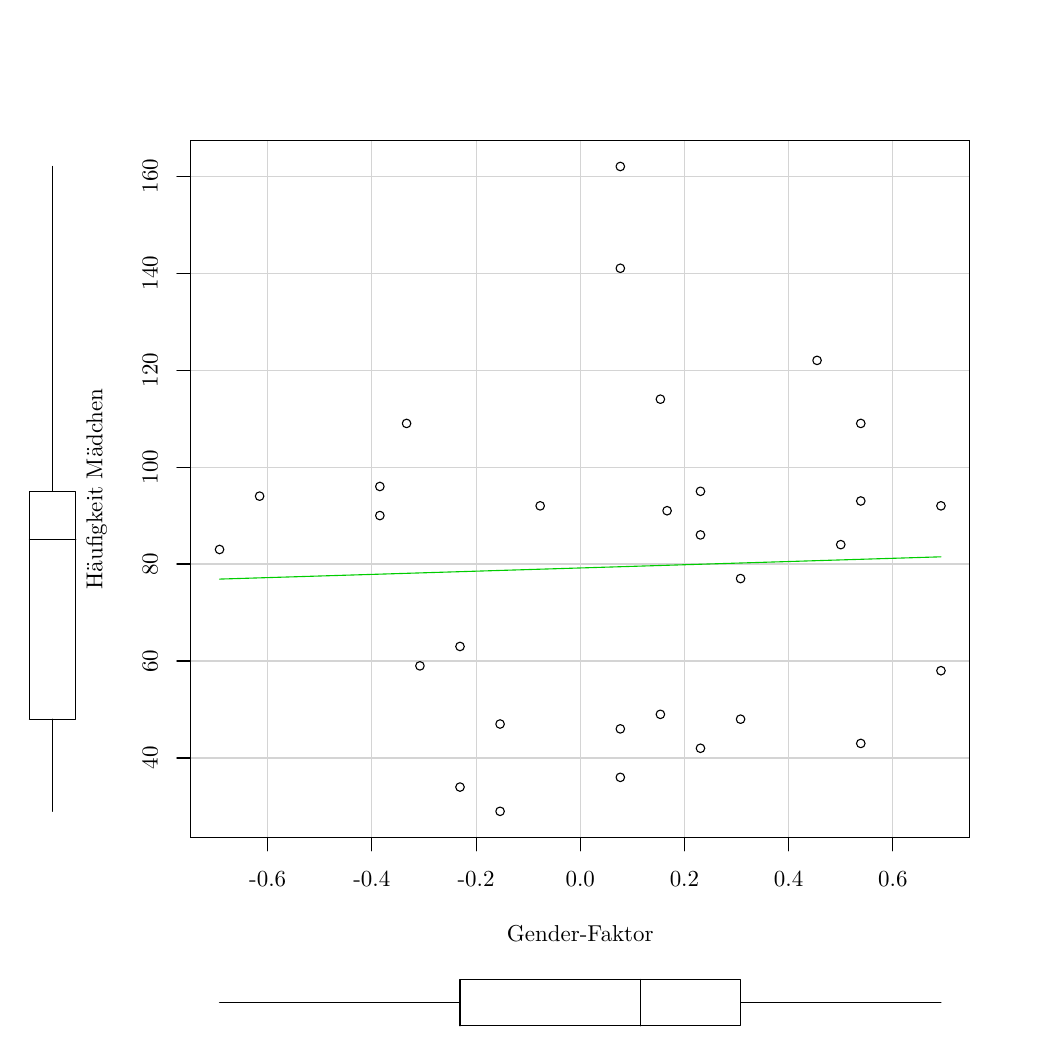
\begin{tikzpicture}[x=1pt,y=1pt]
\definecolor[named]{fillColor}{rgb}{1.00,1.00,1.00}
\path[use as bounding box,fill=fillColor,fill opacity=0.00] (0,0) rectangle (361.35,361.35);
\begin{scope}
\path[clip] (  0.00, 68.86) rectangle ( 18.07,320.51);
\definecolor[named]{drawColor}{rgb}{0.00,0.00,0.00}

\path[draw=drawColor,line width= 0.4pt,line join=round,line cap=round] (  0.67,111.47) --
	( 17.40,111.47) --
	( 17.40,193.81) --
	(  0.67,193.81) --
	(  0.67,111.47);

\path[draw=drawColor,line width= 0.4pt,line join=round,line cap=round] (  0.67,176.29) --
	( 17.40,176.29);

\path[draw=drawColor,line width= 0.4pt,line join=round,line cap=round] (  9.03, 78.18) --
	(  9.03,111.47);

\path[draw=drawColor,line width= 0.4pt,line join=round,line cap=round] (  9.03,193.81) --
	(  9.03,311.19);
\end{scope}
\begin{scope}
\path[clip] ( 58.90,  0.00) rectangle (340.43, 18.07);
\definecolor[named]{drawColor}{rgb}{0.00,0.00,0.00}

\path[draw=drawColor,line width= 0.4pt,line join=round,line cap=round] (156.22,  0.67) --
	(156.22, 17.40) --
	(257.60, 17.40) --
	(257.60,  0.67) --
	(156.22,  0.67);

\path[draw=drawColor,line width= 0.4pt,line join=round,line cap=round] (221.39,  0.67) --
	(221.39, 17.40);

\path[draw=drawColor,line width= 0.4pt,line join=round,line cap=round] ( 69.33,  9.03) --
	(156.22,  9.03);

\path[draw=drawColor,line width= 0.4pt,line join=round,line cap=round] (257.60,  9.03) --
	(330.01,  9.03);
\end{scope}
\begin{scope}
\path[clip] (  0.00,  0.00) rectangle (361.35,361.35);
\definecolor[named]{drawColor}{rgb}{0.00,0.00,0.00}

\path[draw=drawColor,line width= 0.4pt,line join=round,line cap=round] ( 86.71, 68.86) -- (312.63, 68.86);

\path[draw=drawColor,line width= 0.4pt,line join=round,line cap=round] ( 86.71, 68.86) -- ( 86.71, 63.88);

\path[draw=drawColor,line width= 0.4pt,line join=round,line cap=round] (124.36, 68.86) -- (124.36, 63.88);

\path[draw=drawColor,line width= 0.4pt,line join=round,line cap=round] (162.02, 68.86) -- (162.02, 63.88);

\path[draw=drawColor,line width= 0.4pt,line join=round,line cap=round] (199.67, 68.86) -- (199.67, 63.88);

\path[draw=drawColor,line width= 0.4pt,line join=round,line cap=round] (237.32, 68.86) -- (237.32, 63.88);

\path[draw=drawColor,line width= 0.4pt,line join=round,line cap=round] (274.98, 68.86) -- (274.98, 63.88);

\path[draw=drawColor,line width= 0.4pt,line join=round,line cap=round] (312.63, 68.86) -- (312.63, 63.88);

\node[text=drawColor,anchor=base,inner sep=0pt, outer sep=0pt, scale=  0.83] at ( 86.71, 50.94) {-0.6};

\node[text=drawColor,anchor=base,inner sep=0pt, outer sep=0pt, scale=  0.83] at (124.36, 50.94) {-0.4};

\node[text=drawColor,anchor=base,inner sep=0pt, outer sep=0pt, scale=  0.83] at (162.02, 50.94) {-0.2};

\node[text=drawColor,anchor=base,inner sep=0pt, outer sep=0pt, scale=  0.83] at (199.67, 50.94) {0.0};

\node[text=drawColor,anchor=base,inner sep=0pt, outer sep=0pt, scale=  0.83] at (237.32, 50.94) {0.2};

\node[text=drawColor,anchor=base,inner sep=0pt, outer sep=0pt, scale=  0.83] at (274.98, 50.94) {0.4};

\node[text=drawColor,anchor=base,inner sep=0pt, outer sep=0pt, scale=  0.83] at (312.63, 50.94) {0.6};

\path[draw=drawColor,line width= 0.4pt,line join=round,line cap=round] ( 58.90, 97.46) -- ( 58.90,307.69);

\path[draw=drawColor,line width= 0.4pt,line join=round,line cap=round] ( 58.90, 97.46) -- ( 53.92, 97.46);

\path[draw=drawColor,line width= 0.4pt,line join=round,line cap=round] ( 58.90,132.49) -- ( 53.92,132.49);

\path[draw=drawColor,line width= 0.4pt,line join=round,line cap=round] ( 58.90,167.53) -- ( 53.92,167.53);

\path[draw=drawColor,line width= 0.4pt,line join=round,line cap=round] ( 58.90,202.57) -- ( 53.92,202.57);

\path[draw=drawColor,line width= 0.4pt,line join=round,line cap=round] ( 58.90,237.61) -- ( 53.92,237.61);

\path[draw=drawColor,line width= 0.4pt,line join=round,line cap=round] ( 58.90,272.65) -- ( 53.92,272.65);

\path[draw=drawColor,line width= 0.4pt,line join=round,line cap=round] ( 58.90,307.69) -- ( 53.92,307.69);

\node[text=drawColor,rotate= 90.00,anchor=base,inner sep=0pt, outer sep=0pt, scale=  0.83] at ( 46.95, 97.46) {40};

\node[text=drawColor,rotate= 90.00,anchor=base,inner sep=0pt, outer sep=0pt, scale=  0.83] at ( 46.95,132.49) {60};

\node[text=drawColor,rotate= 90.00,anchor=base,inner sep=0pt, outer sep=0pt, scale=  0.83] at ( 46.95,167.53) {80};

\node[text=drawColor,rotate= 90.00,anchor=base,inner sep=0pt, outer sep=0pt, scale=  0.83] at ( 46.95,202.57) {100};

\node[text=drawColor,rotate= 90.00,anchor=base,inner sep=0pt, outer sep=0pt, scale=  0.83] at ( 46.95,237.61) {120};

\node[text=drawColor,rotate= 90.00,anchor=base,inner sep=0pt, outer sep=0pt, scale=  0.83] at ( 46.95,272.65) {140};

\node[text=drawColor,rotate= 90.00,anchor=base,inner sep=0pt, outer sep=0pt, scale=  0.83] at ( 46.95,307.69) {160};

\path[draw=drawColor,line width= 0.4pt,line join=round,line cap=round] ( 58.90, 68.86) --
	(340.43, 68.86) --
	(340.43,320.51) --
	( 58.90,320.51) --
	( 58.90, 68.86);
\end{scope}
\begin{scope}
\path[clip] ( 18.07, 18.07) rectangle (361.35,361.35);
\definecolor[named]{drawColor}{rgb}{0.00,0.00,0.00}

\node[text=drawColor,anchor=base,inner sep=0pt, outer sep=0pt, scale=  0.83] at (199.67, 31.02) {Gender-Faktor};

\node[text=drawColor,rotate= 90.00,anchor=base,inner sep=0pt, outer sep=0pt, scale=  0.83] at ( 27.03,194.69) {Häufigkeit Mädchen};
\end{scope}
\begin{scope}
\path[clip] ( 58.90, 68.86) rectangle (340.43,320.51);
\definecolor[named]{drawColor}{rgb}{0.83,0.83,0.83}

\path[draw=drawColor,line width= 0.4pt,line join=round,line cap=round] ( 86.71, 68.86) -- ( 86.71,320.51);

\path[draw=drawColor,line width= 0.4pt,line join=round,line cap=round] (124.36, 68.86) -- (124.36,320.51);

\path[draw=drawColor,line width= 0.4pt,line join=round,line cap=round] (162.02, 68.86) -- (162.02,320.51);

\path[draw=drawColor,line width= 0.4pt,line join=round,line cap=round] (199.67, 68.86) -- (199.67,320.51);

\path[draw=drawColor,line width= 0.4pt,line join=round,line cap=round] (237.32, 68.86) -- (237.32,320.51);

\path[draw=drawColor,line width= 0.4pt,line join=round,line cap=round] (274.98, 68.86) -- (274.98,320.51);

\path[draw=drawColor,line width= 0.4pt,line join=round,line cap=round] (312.63, 68.86) -- (312.63,320.51);

\path[draw=drawColor,line width= 0.4pt,line join=round,line cap=round] ( 58.90, 97.46) -- (340.43, 97.46);

\path[draw=drawColor,line width= 0.4pt,line join=round,line cap=round] ( 58.90,132.49) -- (340.43,132.49);

\path[draw=drawColor,line width= 0.4pt,line join=round,line cap=round] ( 58.90,167.53) -- (340.43,167.53);

\path[draw=drawColor,line width= 0.4pt,line join=round,line cap=round] ( 58.90,202.57) -- (340.43,202.57);

\path[draw=drawColor,line width= 0.4pt,line join=round,line cap=round] ( 58.90,237.61) -- (340.43,237.61);

\path[draw=drawColor,line width= 0.4pt,line join=round,line cap=round] ( 58.90,272.65) -- (340.43,272.65);

\path[draw=drawColor,line width= 0.4pt,line join=round,line cap=round] ( 58.90,307.69) -- (340.43,307.69);
\end{scope}
\begin{scope}
\path[clip] (  0.00,  0.00) rectangle (361.35,361.35);
\definecolor[named]{drawColor}{rgb}{0.00,0.00,0.00}

\path[draw=drawColor,line width= 0.4pt,line join=round,line cap=round] ( 58.90, 68.86) --
	(340.43, 68.86) --
	(340.43,320.51) --
	( 58.90,320.51) --
	( 58.90, 68.86);
\end{scope}
\begin{scope}
\path[clip] ( 58.90, 68.86) rectangle (340.43,320.51);
\definecolor[named]{drawColor}{rgb}{0.00,0.00,0.00}

\path[draw=drawColor,line width= 0.4pt,line join=round,line cap=round] (214.15,107.97) circle (  1.55);

\path[draw=drawColor,line width= 0.4pt,line join=round,line cap=round] (170.70, 78.18) circle (  1.55);

\path[draw=drawColor,line width= 0.4pt,line join=round,line cap=round] (170.70,109.72) circle (  1.55);

\path[draw=drawColor,line width= 0.4pt,line join=round,line cap=round] (228.63,227.10) circle (  1.55);

\path[draw=drawColor,line width= 0.4pt,line join=round,line cap=round] (228.63,113.22) circle (  1.55);

\path[draw=drawColor,line width= 0.4pt,line join=round,line cap=round] (257.60,111.47) circle (  1.55);

\path[draw=drawColor,line width= 0.4pt,line join=round,line cap=round] (293.80,174.54) circle (  1.55);

\path[draw=drawColor,line width= 0.4pt,line join=round,line cap=round] (136.91,218.34) circle (  1.55);

\path[draw=drawColor,line width= 0.4pt,line join=round,line cap=round] (214.15,311.19) circle (  1.55);

\path[draw=drawColor,line width= 0.4pt,line join=round,line cap=round] ( 83.81,192.06) circle (  1.55);

\path[draw=drawColor,line width= 0.4pt,line join=round,line cap=round] (214.15,274.40) circle (  1.55);

\path[draw=drawColor,line width= 0.4pt,line join=round,line cap=round] (141.74,130.74) circle (  1.55);

\path[draw=drawColor,line width= 0.4pt,line join=round,line cap=round] (257.60,162.28) circle (  1.55);

\path[draw=drawColor,line width= 0.4pt,line join=round,line cap=round] (301.04,218.34) circle (  1.55);

\path[draw=drawColor,line width= 0.4pt,line join=round,line cap=round] (231.05,186.80) circle (  1.55);

\path[draw=drawColor,line width= 0.4pt,line join=round,line cap=round] (156.22, 86.94) circle (  1.55);

\path[draw=drawColor,line width= 0.4pt,line join=round,line cap=round] (214.15, 90.45) circle (  1.55);

\path[draw=drawColor,line width= 0.4pt,line join=round,line cap=round] (185.19,188.56) circle (  1.55);

\path[draw=drawColor,line width= 0.4pt,line join=round,line cap=round] (243.11,100.96) circle (  1.55);

\path[draw=drawColor,line width= 0.4pt,line join=round,line cap=round] (127.26,195.56) circle (  1.55);

\path[draw=drawColor,line width= 0.4pt,line join=round,line cap=round] (330.01,188.56) circle (  1.55);

\path[draw=drawColor,line width= 0.4pt,line join=round,line cap=round] (127.26,185.05) circle (  1.55);

\path[draw=drawColor,line width= 0.4pt,line join=round,line cap=round] (301.04,102.71) circle (  1.55);

\path[draw=drawColor,line width= 0.4pt,line join=round,line cap=round] ( 69.33,172.79) circle (  1.55);

\path[draw=drawColor,line width= 0.4pt,line join=round,line cap=round] (243.11,193.81) circle (  1.55);

\path[draw=drawColor,line width= 0.4pt,line join=round,line cap=round] (301.04,190.31) circle (  1.55);

\path[draw=drawColor,line width= 0.4pt,line join=round,line cap=round] (243.11,178.05) circle (  1.55);

\path[draw=drawColor,line width= 0.4pt,line join=round,line cap=round] (330.01,128.99) circle (  1.55);

\path[draw=drawColor,line width= 0.4pt,line join=round,line cap=round] (285.24,241.12) circle (  1.55);

\path[draw=drawColor,line width= 0.4pt,line join=round,line cap=round] (156.22,137.75) circle (  1.55);
\definecolor[named]{drawColor}{rgb}{0.00,0.80,0.00}

\path[draw=drawColor,line width= 0.4pt,line join=round,line cap=round] ( 69.33,162.09) --
	(330.01,170.14);
\end{scope}
\end{tikzpicture}
